% solution.tex  -- written by Saumya
\section{Proposed Solution}

\subsection{System Architecture}
Fig.~\ref{fig:system} shows the final accelerator
(\texttt{systolic\_top\_v2}); the blocks added in Phase~II are outlined.
The host writes one row of $A$ or $B$ per cycle into the \emph{shadow} bank
of the ping-pong buffers. A \texttt{start} pulse swaps the banks, and the
controller streams column $k$ of $A$ and row $k$ of $B$ into the skew
buffers. The skew buffers stagger them into the diagonal wavefront needed
by the $4\times4$ PE array. On completion the accumulators are copied into a
result buffer, from which the host reads one row of $C$ per cycle, either
raw (Q24.8) or requantised (Q4.4). Table~\ref{tab:modules} lists the RTL
hierarchy. The Phase~I top level (\texttt{systolic\_top}) is kept unchanged
as a comparison point.

\begin{figure*}[t]
\centering
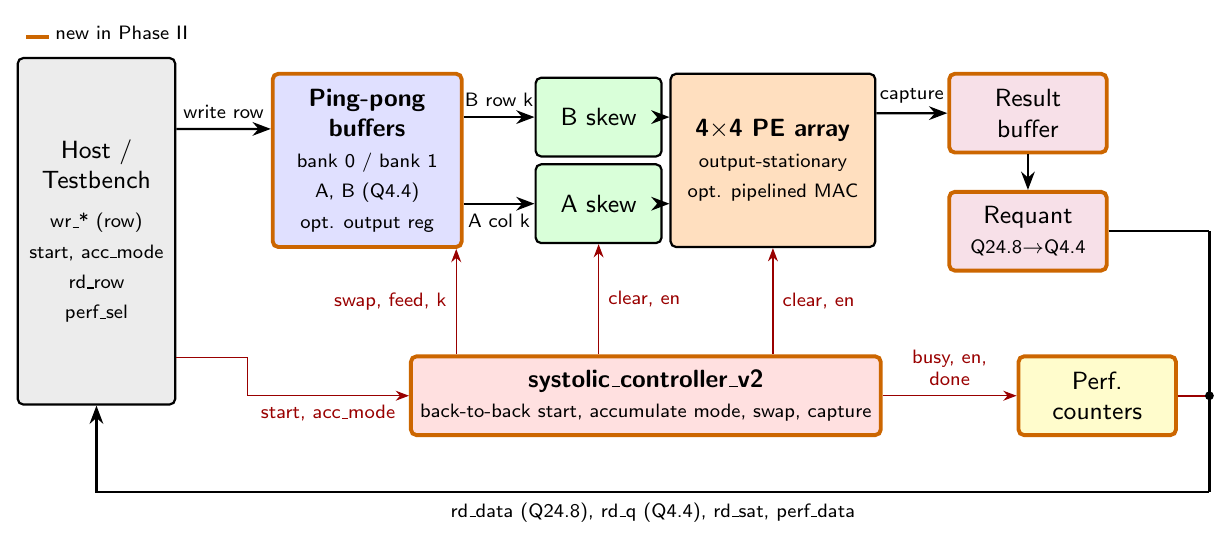
\includegraphics[width=0.86\textwidth]{fig_system_v2.png}
\caption{Final accelerator \texttt{systolic\_top\_v2}. Orange outlines mark blocks added in Phase~II.}
\label{fig:system}
\end{figure*}

\begin{table}[t]
\centering
\caption{RTL modules (Verilog-2005)}
\label{tab:modules}
\setlength{\tabcolsep}{2.5pt}
\begin{tabular}{@{}lp{4.75cm}@{}}
\toprule
\textbf{Module} & \textbf{Function} \\
\midrule
\texttt{mac\_unit} & Q4.4$\times$Q4.4 MAC, 32-bit acc., opt.\ pipeline \\
\texttt{pe} & MAC + east/south forwarding registers \\
\texttt{systolic\_array} & $N\times N$ PE grid (\texttt{generate}) \\
\texttt{input\_skew} & lane $k$ delayed by $k$ cycles \\
\texttt{matrix\_buffer\_pp} & ping-pong $A$/$B$ banks, row writes \\
\texttt{systolic\_controller\_v2} & FSM: back-to-back, accumulate, swap \\
\texttt{requant} & Q24.8$\to$Q4.4, round + saturate \\
\texttt{perf\_counters} & cycle / busy / product counters \\
\texttt{systolic\_top\_v2} & integration + result buffer \\
\midrule
\texttt{seq\_matmul} & baseline: one MAC, $N^3$ cycles \\
\texttt{pe\_ws}, \texttt{ws\_top} & weight-stationary streaming array \\
\texttt{systolic\_top} & Phase~I top (element-wise interface) \\
\bottomrule
\end{tabular}
\end{table}

\subsection{Number Representation and Requantisation}
Operands are signed Q4.4 (range $[-8, 7.9375]$, resolution $0.0625$).
Their product is exact in Q8.8 and is sign-extended into a 32-bit Q24.8
accumulator. For $N\le 16$ the worst case $16\cdot128\cdot128 = 2^{18}$
cannot overflow. The \texttt{requant} block converts a result back to the
operand format so it can feed the next layer. It adds half an output LSB
($2^{3}$), shifts right arithmetically by 4 bits, and clamps to
$[-128,127]$, raising a per-lane \texttt{sat} flag when it clamps
(round-half-up, the same rule as the golden model). For example,
$\texttt{872}/256 = 3.406$ becomes $55/16 = 3.4375$.

\subsection{MAC Unit and Processing Element}
The PE (Fig.~\ref{fig:pe}) wraps one MAC and two forwarding registers. $A$
moves east and $B$ moves south, one PE per cycle, while the local
accumulator builds $C_{ij}$. With \texttt{MUL\_PIPE}=1 the product,
\texttt{en} and \texttt{clear} are registered before the adder. This splits
the multiply-add path at the cost of one cycle of latency, and throughput
stays one MAC per cycle.

\begin{figure}[t]
\centering
\includegraphics[width=0.82\columnwidth]{fig_pe.png}
\caption{Output-stationary PE (Phase~I) with the MAC unit.}
\label{fig:pe}
\end{figure}

\subsection{Array Organisation and Data Skew}
\texttt{systolic\_array} instantiates $N^2$ PEs in nested \texttt{generate}
loops. Row $i$ of $A$ and column $j$ of $B$ are delayed by $i$ and $j$
cycles (Fig.~\ref{fig:dataflow}), so $a_{ik}$ and $b_{kj}$ meet in
PE$(i,j)$ at cycle
\begin{equation}
t_{\text{meet}}(i,j,k) = k + i + j .
\end{equation}
The last pair reaches PE$(N\!-\!1,N\!-\!1)$ at $t=3N-3$, so a product needs
$N$ feed cycles and $2N-2$ drain cycles.

\begin{figure}[t]
\centering
\includegraphics[width=0.9\columnwidth]{fig_dataflow.png}
\caption{Skewed input wavefront: $A$ rows delayed by $i$, $B$ columns by $j$ cycles.}
\label{fig:dataflow}
\end{figure}

\subsection{Ping-pong Buffers, Result Buffer and Host Interface}
Phase~I moved one element per cycle, so loading two $4\times4$ matrices
took 32 cycles and reading the result took 16, while the computation took
only 12. Phase~II makes the interface \emph{row-wide} (32-bit write, 128-bit
read). It also duplicates the operand storage into two banks:
\texttt{swap} flips which bank the array reads, so the host can fill the
other bank during a computation. The \texttt{capture} pulse copies the
16 accumulators into a 512-bit result buffer, so results stay readable
while the next product runs. An optional output register on the buffer
(\texttt{BUF\_REG}) removes the read multiplexer from the critical path.

\subsection{Controller}
The controller keeps the five Phase~I states (Fig.~\ref{fig:fsm}) and
adds four features. First, \texttt{start} is accepted in \textsc{Done}
as well as \textsc{Idle}, so products run back to back with no idle
cycle. Second, \texttt{acc\_mode} skips \textsc{Clear}, so a new product
adds onto the previous result; this is used for tiling. Third, it
generates the \texttt{swap} pulse, and fourth, the \texttt{capture} pulse.
\textsc{Drain} lasts $2N-2+\texttt{MUL\_PIPE}+\texttt{BUF\_REG}$ cycles.

\begin{figure}[t]
\centering
\includegraphics[width=\columnwidth]{fig_fsm.png}
\caption{Controller states (Phase~I). Phase~II adds the \textsc{Done}$\to$\textsc{Clear}/\textsc{Feed} transitions and the accumulate path.}
\label{fig:fsm}
\end{figure}

\subsection{Performance Counters}
Four 32-bit counters (total cycles, busy cycles, array-advance cycles and
completed products) let the testbench measure the hardware from inside.
This is the accelerator equivalent of CPU cycle and instruction counters,
and it gives cycles per product and PE utilisation
($= \text{products}\cdot N^3 / (N^2\cdot\text{cycles})$).

\subsection{Comparison Designs}
\emph{Sequential baseline} (\texttt{seq\_matmul}): a single MAC executes the
$i,j,k$ triple loop in exactly $N^3$ cycles. Operands and results are kept
in small memories, as in a simple CPU. It has the same host interface as
the Phase~I top, so the same testbench verifies both.

\emph{Weight-stationary array} (\texttt{ws\_top}): each PE holds $B_{kj}$,
loaded by shifting rows down the columns for $N$ cycles. Rows of $A$ then
stream in continuously. The 32-bit partial sums flow south, and row $i$ of
$C$ leaves the bottom after $2N-1$ cycles. Output skew is removed by
reusing \texttt{input\_skew} on reversed lanes.

\subsection{Verification and Implementation Flow}
Every testbench is self-checking and fails loudly if its vector file is
missing. A pure-Python golden model reproduces the hardware arithmetic
bit for bit, including requantisation. It generates directed, random,
requantisation, WS and tiling vectors. Simulation uses Icarus
Verilog~\cite{icarus} (Verilog-2005~\cite{ieee1364}). Synthesis uses
Yosys~\cite{wolf_yosys}: \texttt{synth\_xilinx} gives Xilinx 7-series resource
estimates, and \texttt{synth\_ecp5} followed by nextpnr place-and-route on a
Lattice ECP5-85F gives post-route $f_{\max}$.
